\documentclass[11pt]{article}

\usepackage[margin=1.0in]{geometry}
%\linespread{1.5}
\usepackage{graphicx}
\usepackage{natbib}
\usepackage{amsmath}
\usepackage{fancyhdr}
\usepackage{changepage}
\usepackage{rotating}
\sloppy

\pdfminorversion 4

\bibpunct[,]{(}{)}{;}{a}{}{,}


\renewcommand{\bottomfraction}{.9}
\renewcommand{\topfraction}{.9}
\renewcommand{\textfraction}{0.1}
\renewcommand{\floatpagefraction}{.9}




\fancypagestyle{plain}{%
   \fancyhead[R]{\fbox{\big{\textbf{Letter}}}}
   \renewcommand{\headrulewidth}{0pt}
}


\begin{document}

\title{\textbf{Limited utility of residue masking for positive-selection inference}}
\author{Stephanie J. Spielman$^{1*}$ and Eric T. Dawson$^{1}$ and Claus O. Wilke$^{1}$}
\date{}

\maketitle
\noindent
Address:\\
$^1$Department of Integrative Biology, Center for Computational Biology and Bioinformatics, and Institute of Cellular and Molecular Biology.
The University of Texas at Austin, Austin, TX 78712, USA.\\

\bigskip
\noindent
$^*$Corresponding author\\
$\phantom{^*}$Email: stephanie.spielman@utexas.edu\\

\bigskip
\noindent
Manuscript type: Letter

\bigskip
\noindent Keywords: multiple sequence alignment, alignment filters, positive-selection inference, sequence simulation

\newpage
\begin{abstract}
Multiple sequence alignment (MSA) errors are known to reduce accuracy in positive-selection inference. In response to this issue, some have suggested filtering MSAs before conducting further analyses. One widely-used filter, Guidance, generates site-specific MSA confidence scores, allowing users to remove positions of low confidence. Studies investigating this filter's utility for positive-selection inference have yielded inconsistent results; some have demonstrated that Guidance substantially improved accuracy, but others have found that Guidance affected accuracy minimally. Motivated by these discrepancies, we have conducted a extensive simulation-based study to characterize how Guidance impacts positive-selection inference. We particularly investigated whether novel scoring algorithms, which phylogenetically corrected confidence scores, and a new gap-penalization score-normalization scheme improved upon Guidance's performance. Instead, we found that no filter, including the original Guidance, consistently improved positive-selection inference across multiple inference methods. Moreover, all improvements detected were of exceedingly small magnitude, and in certain circumstances, MSA filters worsened positive-selection inference. %149 words! huzzah!
\end{abstract}


Constructing a multiple sequence alignment (MSA) represents the most fundamental step in most molecular evolution studies, including phylogenetic reconstruction and evolutionary rate inference. Recently, several studies have shown that poor MSA quality can hinder accuracy in positive-selection inference  \citep{Schneider2009, Fletcher2010, MarkovaRaina2011}. As a consequence, some have advocated that users filter MSAs before subsequent analyses to remove putatively-poorly aligned regions \citep{Privman2012,Jordan2012}, thereby reducing noise and maximizing signal in the MSA.

One filter, known as Guidance \citep{Penn2010}, is widely used in positive-selection inference. Guidance derives a confidence score for each MSA position by sampling variants in the guide tree used to construct progressive alignments. Using these confidence scores, users can mask positions that score below a set threshold, effectively removing residues that may produce misleading signal. Unfortunately, studies investigating Guidance's utility in positive-selection inference have produced conflicting findings. While one study by \citet{Privman2012} found that Guidance dramatically improved accuracy, a separate study by \citet{Jordan2012} found that Guidance affected positive-selection inference modestly, if at all. In particular, both \citet{Privman2012} and \citet{Jordan2012} concluded that Guidance filtering improved inference primarily at high insertion/deletion (indel) rates (e.g. 10\%) and/or high divergence levels (e.g. mean-path-length of 1.8). However, it is important to recognize that typical positive-selection studies rarely contain sequences separated by such high divergences, so it remains unclear how useful Guidance filtering is at average divergence levels.

In sum, \citet{Privman2012} strongly advocated Guidance's use, while \citet{Jordan2012} emphasized relying primarily on robust MSA construction methods. To reconcile these distinct recommendations, we have conducted an extensive simulation-based study to elucidate how the Guidance filter affects positive-selection inference. In particular, we examined the potential benefits to modifying the Guidance scoring scheme in several ways.  First, we assessed whether two novel algorithms that corrected Guidance scores for the sequences' phylogenetic relationships could improve upon the original Guidance algorithm. Briefly, the first phylogenetically-corrected method incorporated a weight, as calculated by BranchManager \citep{Stone2007}, for each MSA sequence, and the second method incorporated patristic distances (the sum of branch lengths between two taxa), as calculated through the Python phylogenetics library Dendropy \citep{Sukumaran2010}. We refer to these methods, respectively, BMweights and PDweights. Moreover, we tested a new gap-penalization score-normalization scheme, which scales a given residue's score according to the number of gaps in its column. This strategy naturally assigned lower scores to residues in gappy columns, thereby capturing the inherent unreliability of such regions. We refer to filters using the gap-penalization scheme as GuidanceP, BMweightsP, and PDweightsP. To assess the performance of these novel algorithms, we reimplemented the Guidance software (available at https://github.com/clauswilke/alignment\underline{\hspace*{0.2cm}}filtering). 

We simulated protein-coding sequences using Indelible \citep{Fletcher2009} according to two different selective profiles: H1N1 influenza hemagluttinin (HA), which featured a mean $dN/dS = 0.37$, and HIV-1 envelope protein subunit GP41, which featured a mean $dN/dS = 0.89$. We used these two selective profiles because, while both genes are known to contain positively selected regions \citep{Bush1999, Frost2001, Bandawe2008, Meyer2012}, the majority of sites in HA are either under strong purifying or positive selection, whereas GP41  contains a much larger proportion of sites near neutral, making positive-selection inference more challenging. For each selective profile, we simulated 100 MSA replicates along each of four different gene trees consisting of 11 \citep{Spielman2013}, 26 \citep{Spielman2013}, 60 \citep{Yang2011}, and 158 \citep{Betancur2013} taxa, yielding a total of 800 simulated MSAs. All sequences were simulated with a 5\% indel rate, which has been shown to be typical of mammalian genomes \citep{Cooper2004}.

We processed the unaligned amino-acid sequences with our Guidance reimplementation using the aligner MAFFT L-INS-I (linsi) \citep{Katoh2002,Katoh2005} and calculated confidence scores for all inferred MSAs using each of the six scoring algorithms detailed above. When filtering MSAs with Guidance-based methods, one must select a specific score cutoff below which to mask residues. We investigated any potential differences resulting from the four masking cutoffs 0.3, 0.5, 0.7, and 0.9 (see Supplementary Materials for details), and found that the 0.9 cutoff, at times, performed much worse than did the other cutoffs, which performed similarly to one another (Table S1). Therefore, we masked positions with scores below 0.5, the same threshold as used by \citet{Jordan2012}. 

We used two methods to infer positive selection: FUBAR \citep{Murrell2013}, as implemented in HyPhy \citep{Pond2005}, and the widely-used M8 model in PAML \citep{Yang2000, Yang2007}. Phylogenies used during positive-selection inference were constructed in RAxMLv7.3.0 using the ``PROTGAMMAWAG" model \citep{Stamatakis2006}.  Note that while we processed all MSAs with FUBAR, we did not infer positive selection with PAML for MSAs of 158 taxa due to prohibitive runtimes. A detailed description of all methods, including the Guidance software reimplementation, is available in Supplementary Material.


\subsection*{Guidance-based filters have a minimal effect on positive-selection inference}

We first compared the resulting true positive rates (TPRs) of positive-selection inference between each filtered MSA and its corresponding unfiltered MSA. We chose to primarily compare the TPRs, as opposed to the false positive rates (FPRs), as the FPRs we recovered were exceedingly small, never surpassing an average of 1\% across simulation sets and inference methods. TPRs were calculated using the true evolutionary rates assigned during sequence simulation. For this analysis, we considered sites to be positively selected if the given inference method (i.e. FUBAR or PAML) returned a posterior probability $\geq0.90$. For each simulation set, we fit a series of mixed-effects models using the R package lme4 \citep{Bates2012}. Each model consisted of TPR as the response variable, filtering algorithm (including unfiltered and the six filtering algorithms) as a fixed effect, and simulation count as a random effect, which accounted for the paired structure of our analysis. 

Table \ref{tab:summarystats} highlights key findings from these models, as well as some additional information regarding the simulated sequences. We found that, in general, there was no significant mean TPR difference among filters within a given normalization scheme. In other words, Guidance, BMweights, and PDweights performed similarly to one another, as did the gap-penalization filtering algorithms. Therefore, Table \ref{tab:summarystats} displays results for only Guidance and GuidanceP (refer to Table S2 for model results from all filtering algorithms). Table \ref{tab:summarystats} demonstrates that, for the majority of datasets studied here, Guidance-based filtering had no significant effect on the mean TPR, relative to an unfiltered MSA. However, in several cases, MSA filtering did significantly increase mean TPR, but in other cases MSA filtering significantly decreased mean TPR. Importantly, for all cases in which MSA filtering significantly changed mean TPR, the change was rather small. 

Moreover, inference methods did not respond to MSA filtering consistently, as demonstrated in Figure~\ref{barplot}, which gives a graphical representation of the linear models' results for the 26- and 60-sequence simulation sets, for both HA and GP41 selective profiles. On one hand, FUBAR yielded consistent mean TPR trends among filters (Guidance mean TPR was generally higher than were both unfiltered and GuidanceP), but this trend was mostly statistically insignificant. PAML's behavior in response to MSA filtering, on the other hand, varied substantially among simulation conditions. For instance, the largest TPR improvement we recovered in this study was for the HA 26-sequence simulation set; when PAML inferred positive-selection on GuidanceP-filtered MSAs, TPR increased by roughly 4\% the TPR for unfiltered MSAs. However, GuidanceP significantly reduced mean TPR for the GP41 60-sequence simulation set, also as inferred with PAML. Therefore, there does not appear to be a strong universal trend dictating when MSA filtering will be helpful. We do note, however, that the GuidanceP filter was more likely to reduce mean TPR than was the Guidance filter, which only significantly reduced TPR in one case (Table \ref{tab:summarystats}). 

We do, however, emphasize that all Guidance-based filters improved positive-selection inference for the largest simulation sets of 158 taxa when analyzed with FUBAR, although the effect magnitude was very small. As we did not analyze these data sets with PAML, we caution this result may not be easily extrapolated to inference methods other than FUBAR. Conversely all filters significantly reduced accuracy for the GP41 11-sequence simulation set, as analyzed with PAML. Taken together, these results suggested that filtering may have some minor benefits large ($geq$ 100 sequences) MSAs, but may remove excessive information from relatively smaller MSAs.

We additionally used receiver operating characteristic (ROC) curves, commonly used to evaluate the performance of binary classification methods, to qualitatively assess whether MSA filtering influences power in positive-selection inference. Importantly, this analysis did not bias results to those obtained from a single posterior probability threshold for calling positive-selected sites, but instead considered the overall methodological performance. ROC curves for the HA and GP41 60-sequence simulation sets are shown in Figure~\ref{roc}. In each sub-plot, the top curve gives results from the HA selective profile, and the bottom curve gives results from the GP41 selective profile. The left-hand panels display the entire ROC curves, while the right-hand panels display only the region of the curves with relatively low FPRs. 

Several trends emerge from Figure~\ref{roc}. First, power in positive-selection inference for HA simulation sets was universally greater than for GP41 simulation sets. This result was largely expected, given that the GP41 selective profile featured a greater proportion of sites with $dN/dS$ near 1, which are more difficult to classify. Even so, Guidance-based filters exhibited consistent behaviors across all simulation conditions. Second, as all algorithms within a given normalization scheme (original vs. gap-penalization) have nearly identical curves, this analysis confirmed that introducing phylogenetically-weighted scores had a minimal, if any, effect on Guidance scores. Finally, across the entire span of the ROC curves, no dramatic difference in area between curves for the unfiltered and filtered MSAs existed, although, MSAs processed with gap-penalization algorithms did, at certain FPR levels (roughly 0.1--0.3), performed worse than did both unfiltered and Guidance-filtered MSAs. Even so, filtering did confer substantial power boosts at low FPR rates, as seen in the right-hand panels, in particular when PAML was used as the inference method. These benefits, unfortunately, were only present at FPR levels of roughly 1\% - 4\%, above which any benefits quickly dissipated. Outside of this narrow FPR region, filtered MSAs either yielded results comparable to or worse than those of unfiltered MSAs. Importantly, our linear models which considered positively-selected sites only at a $0.9$ posterior probability threshold all yielded mean FPRs under 1\%, below the region where MSA filtering increases power. Our low recovered FPRs explained why we did not detect substantial benefits to MSA-filtering through our linear models. ROC curves for all other simulation sets are available in Figures S1 and S2, and yielded broadly consistent results to those described here.


\subsection*{Discussion and Conclusions}

The primary goal of using the Guidance, or similar, MSA filters is to remove excessive noise while maintaining informative data. Ideally, our study would have recovered a clear set of circumstances for which Guidance-based filters could consistently achieve this goal. Instead, we were unable to recover any universal trend to ensure that filtering will only remove noise without potentially compromising valuable data. While Guidance-based filters did improve positive-selection inference under certain conditions, they also diminished power to detect positively selected sites under other circumstances. Therefore, while Guidance-based filtering certainly had the potential to boost power, there was no apparent way to predict whether a given data set would experience this benefit, or worse, have valuable information removed.  Importantly, results from our ROC curves showed that Guidance-based MSA filtering only conferred substantial power increases in an extremely limited region, demonstrating that the method was not robust to varying FPR levels.

Our study focused primarily on divergence levels representative of realistic protein-coding data typically used in positive-selection inference. It is possible that we were unable to recover some of the stronger benefits to Guidance filters when applied to highly diverged data. However, as seen in Table \ref{tab:summarystats}, our MSAs contained gaps in up to 60\% of columns, meaning that constructing MSAs on our datasets was not a trivial task, and portions which were difficult to align certainly existed (Table S2). Again, a given positive-selection study is unlikely to feature a higher proportion of indels than our MSAs, but should such a situation arise, it is possible that Guidance filtering will have a more substantial effect \citep{Privman2012}.

We additionally found that, for nearly all simulation cases, FUBAR outperformed PAML both in TPR and runtime. Each FUBAR inference completed in under 20 minutes, but a single PAML inference took between two hours and a week to complete. FUBAR, therefore, represents a fast and and accurate alternative to traditional positive-selection inference methods.

%Interestingly, incorporating phylogenetic information into the scoring algorithm generally performed the same as did the original Guidance algorithm. This result indicated the minimal benefits that MSA filtering in this manner produced at all. Were the original Guidance to offer robust improvements in positive-selection detection, one might expect that our more statistically controlled approach would boost the method's performance. However, as we have found that masking individual positions in an MSA only marginally affected positive-selection inference in the first place, the algorithmic changes we implemented might not be expected to have a dramatic effect.

Two primary conclusions may be drawn from our study. First, although Guidance did not universally benefit positive-selection inference, it never precluded the detection of positively-selected sites. Therefore, MSA filtering might be regarded as a conservative method in the positive-selection inference pipeline. Alternatively, all benefits that Guidance-based filtering conferred were minimal, and filters behaved inconsistently across simulation sets and selection inference methods. Given these observations, there is no clear way to predict whether MSA filtering will benefit or harm a given analysis, and it very is possible that filtering MSAs with a Guidance-based strategy could inadvertently result in a loss of power. We conclude that, while potentially beneficial, Guidance does not seem to be a particularly robust method for positive-selection inference, and it does not need to be a requisite step in sequence analyses.

In sum, we recommend that users employ high-quality MSA inference (e.g. linsi \citep{Katoh2005} or PRANK \citep{Loytynoja2008}) and positive-selection inference (e.g. FUBAR) methods, in which error can be minimized as much as possible without necessitating post-hoc correction. Moreover, should users decide to filter their MSAs, we recommend using a lenient cutoff ($\leq0.5$) to avoid potentially removing signal.


\subsection*{Acknowledgements}
This work was supported in part by ARO Grant W911NF-12-1-0390 and in part by the National Institutes of Health grant R01 GM088344 to COW. This material is based in part upon work supported by the National Science Foundation under Cooperative Agreement No. DBI-0939454. Any opinions, findings, and conclusions or recommendations expressed in this material are those of the author(s) and do not necessarily reflect the views of the National Science Foundation. The authors thank Eyal Privman for MS comments and Sergei L Kosakovsky Pond for helpful comments and FUBAR(?).


\bibliographystyle{MBE}
\bibliography{citations}	

\newpage

\begin{table}[htbp]
\begin{adjustwidth}{-1cm}{}
\caption {\label{tab:summarystats} Summary statistics for effect of masking.}
\begin{tabular}{l l l c c c c c}
\hline\noalign{\smallskip}
& & & \multicolumn{4}{c}{Mean True Positive Rate} \\
\cline{4-7}\noalign{\smallskip}
\multicolumn{1}{p{1.5cm}}{\centering Selective \\ Profile} & \multicolumn{1}{p{1.5cm}}{\centering Number \\ of Taxa} & \multicolumn{1}{p{1.5cm}}{\centering Inference \\ Method} & \multicolumn{1}{c}{True} & \multicolumn{1}{c}{Unfiltered} & \multicolumn{1}{c}{Guidance} & \multicolumn{1}{c}{GuidanceP} & \multicolumn{1}{c}{Percent Gaps} \\
\noalign{\smallskip}\hline\noalign{\smallskip}
HA  &  11  &  FUBAR  &  0.093  &  0.084  & 0.085 (1.33\%)  &  0.085 (0.74\%) & 11.9\% \\
  &    &  PAML  &  0.086  &  0.082  & 0.081 (-0.48\%)  &  0.081 (-0.60\%) &\\

 & 26 & FUBAR & 0.252 & 0.227 & 0.229 (0.84\%) & 0.226 (-0.38\%) & 26.0\%\\
 &   & PAML & 0.209 & 0.176 & \textbf{0.178 (1.36\%)$^{\ast\ast}$} & \textbf{0.183 (4.04\%)$^{\ast\ast}$} &\\

 & 60 & FUBAR & 0.551 & 0.474 & 0.479 (0.99\%) & \textbf{0.464 (-2.16\%)$^{\ast}$} & 59.4\%\\
 &  & PAML & 0.422 & 0.347 & 0.342 (-1.68\%) & 0.337 (-2.92\%) &\\

 & 158 & FUBAR & 0.515 & 0.458 & \textbf{0.467 (1.89\%)$^{\ast}$} & \textbf{0.468 (2.12\%)$^{\ast}$} & 50.5\%\\
\noalign{\smallskip}\hline\noalign{\smallskip}
GP41  &  11 &  FUBAR  &  0.062  &  0.058  &  0.057 (-1.55\%)  &  0.057 (-1.21\%) & 11.6\%\\
  &    &  PAML  &  0.096  &  0.098  & \textbf{0.095 (-3.49\%)$^{\ast\ast}$}  &  \textbf{0.095 (-3.80\%)$^{\ast\ast}$} &\\

 & 26 & FUBAR & 0.216 & 0.196 & \textbf{0.20 (1.89\%)$^{\ast}$} & 0.197 (0.36\%) & 31.3\%\\
 & & PAML & 0.237 & 0.216 & 0.220 (1.54\%) & 0.217 (0.244\%) &\\

 & 60 & FUBAR & 0.359 & 0.308 & \textbf{0.313 (1.77\%)$^{\ast}$} & 0.304 (-1.16\%) & 58.1\%\\
 & & PAML & 0.341 & 0.304 &0.302 (-0.77\%) & \textbf{0.296 (-2.71\%)$^{\ast\ast}$} & \\

 & 158 & FUBAR & 0.348 & 0.320 & \textbf{0.325 (1.77\%)$^{\ast\ast}$} & \textbf{0.326 (2.02\%)$^{\ast\ast}$} & 48.4\% \\
\noalign{\smallskip}\hline\noalign{\smallskip}
\end{tabular}
\newline
\textsc{note.}--- Mean TPR values shown in bold represent those which are significantly different from the respective unfiltered MSA mean TPR. Values shown in parentheses refer to the average TPR percent change of the respective unfiltered MSA, not the absolute TPR increase or decrease. Significance levels:  $^{\ast\ast} P < 0.001$; $^{\ast} P < 0.01$. All significance levels were corrected for multiple comparisons using the R multcomp package \citep{Hothorn2008}. Note that the true MSAs were not included in the linear models but are shown here for comparative purposes. Percent gaps were calculated from unfiltered alignments as the total number of gaps divided by the total number of MSA positions, and represents the percentage of columns with at least one gap.
\end{adjustwidth}
\end{table}

\begin{figure*}[H]
\centerline{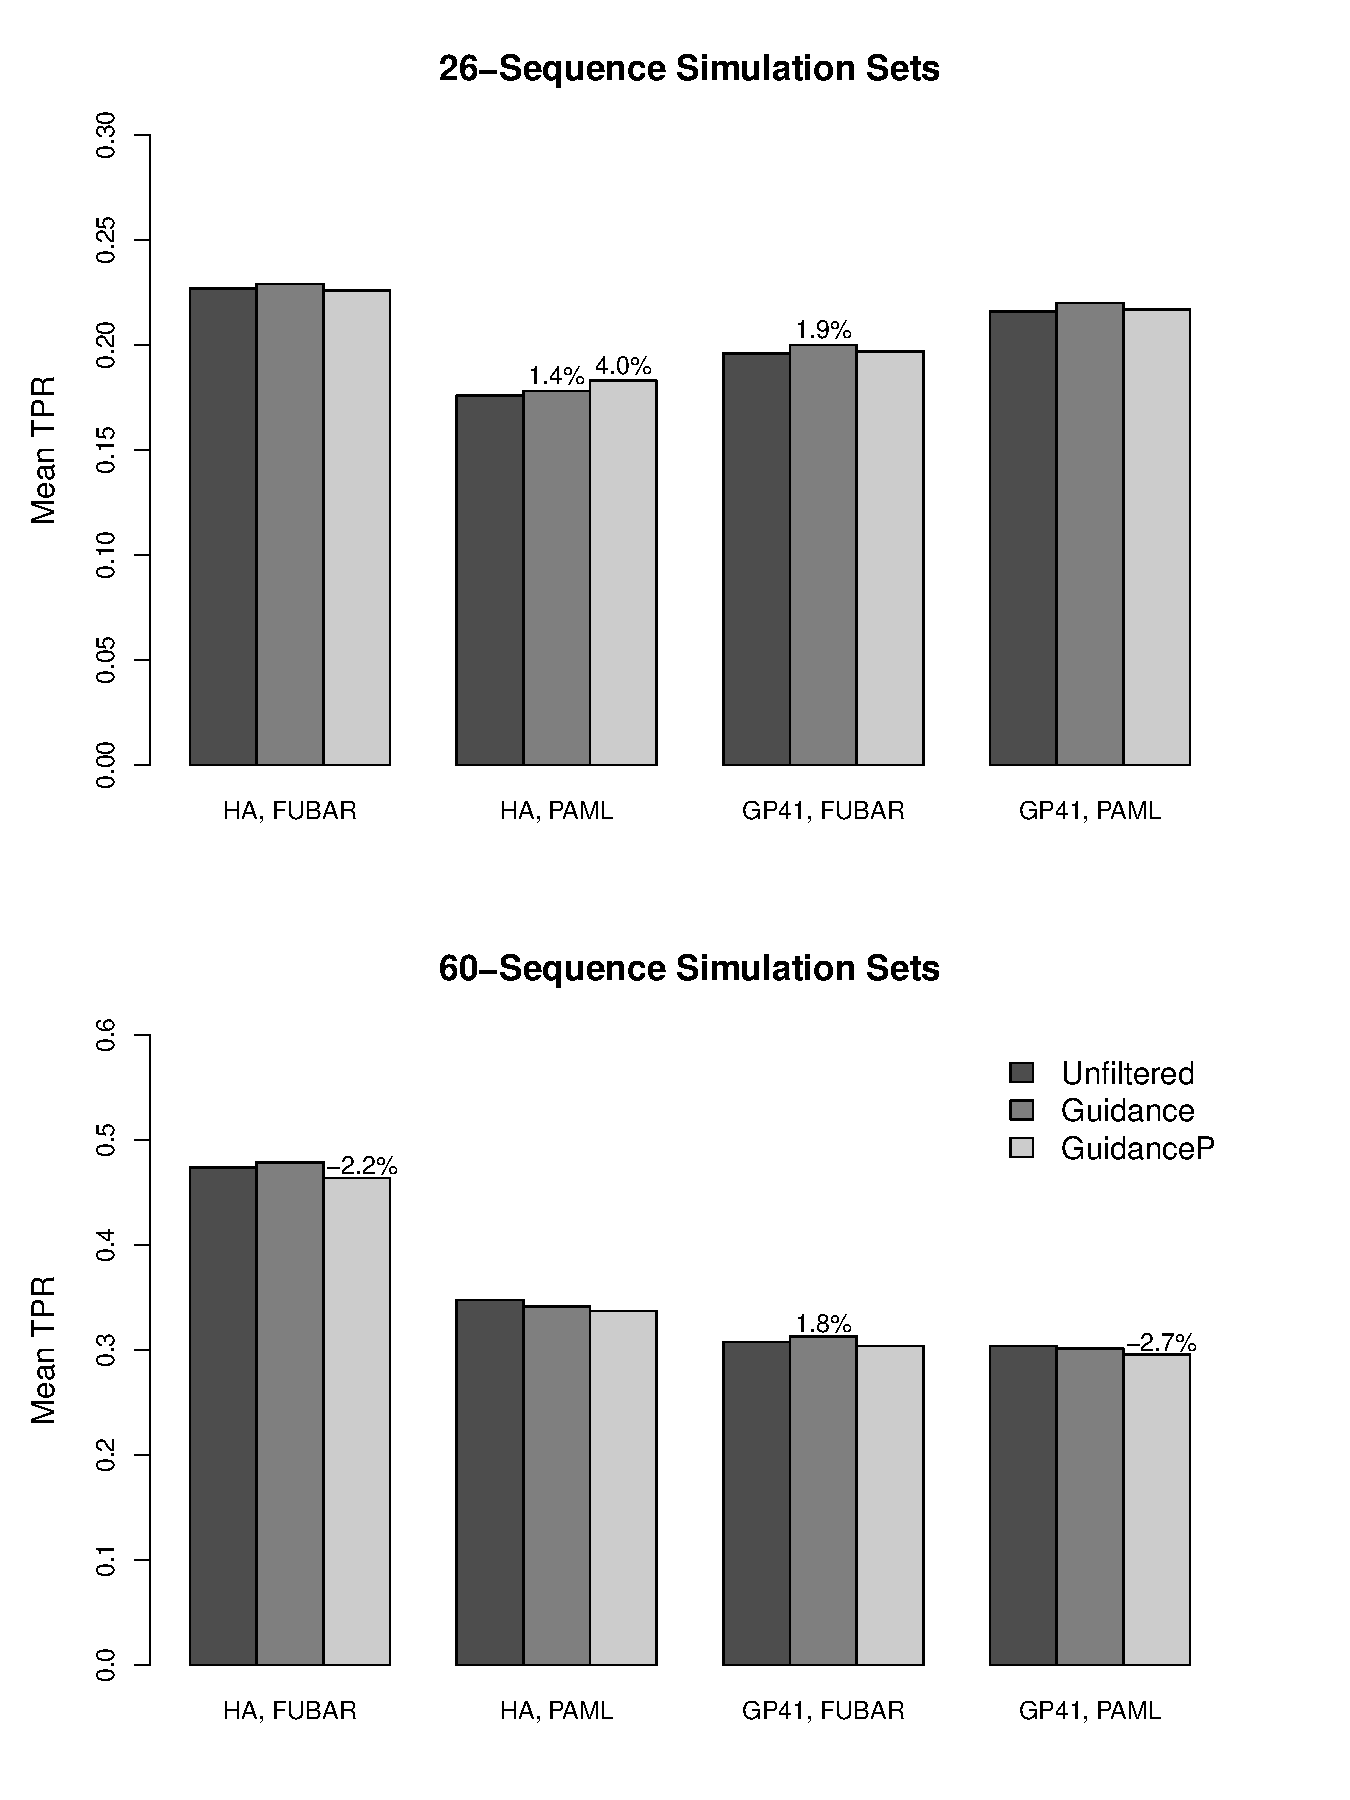
\includegraphics[width=4.75in]{Figures/barplot.pdf}}
\caption{\label{barplot} Mean TPR for and 26- and  60-sequence simulation sets. Percentages, which represent the average percent TPR change relative to the unfiltered MSAs, are shown only for those changes which are significant. Significance levels are the same as those given in Table \ref{tab:summarystats}. Dark gray bars represent unfiltered MSAs, medium gray bars represents MSAs filtered with Guidance, and light gray bars represent MSAs filtered with GuidanceP.}
\end{figure*}

\bigskip

\begin{figure*}[H]
\centerline{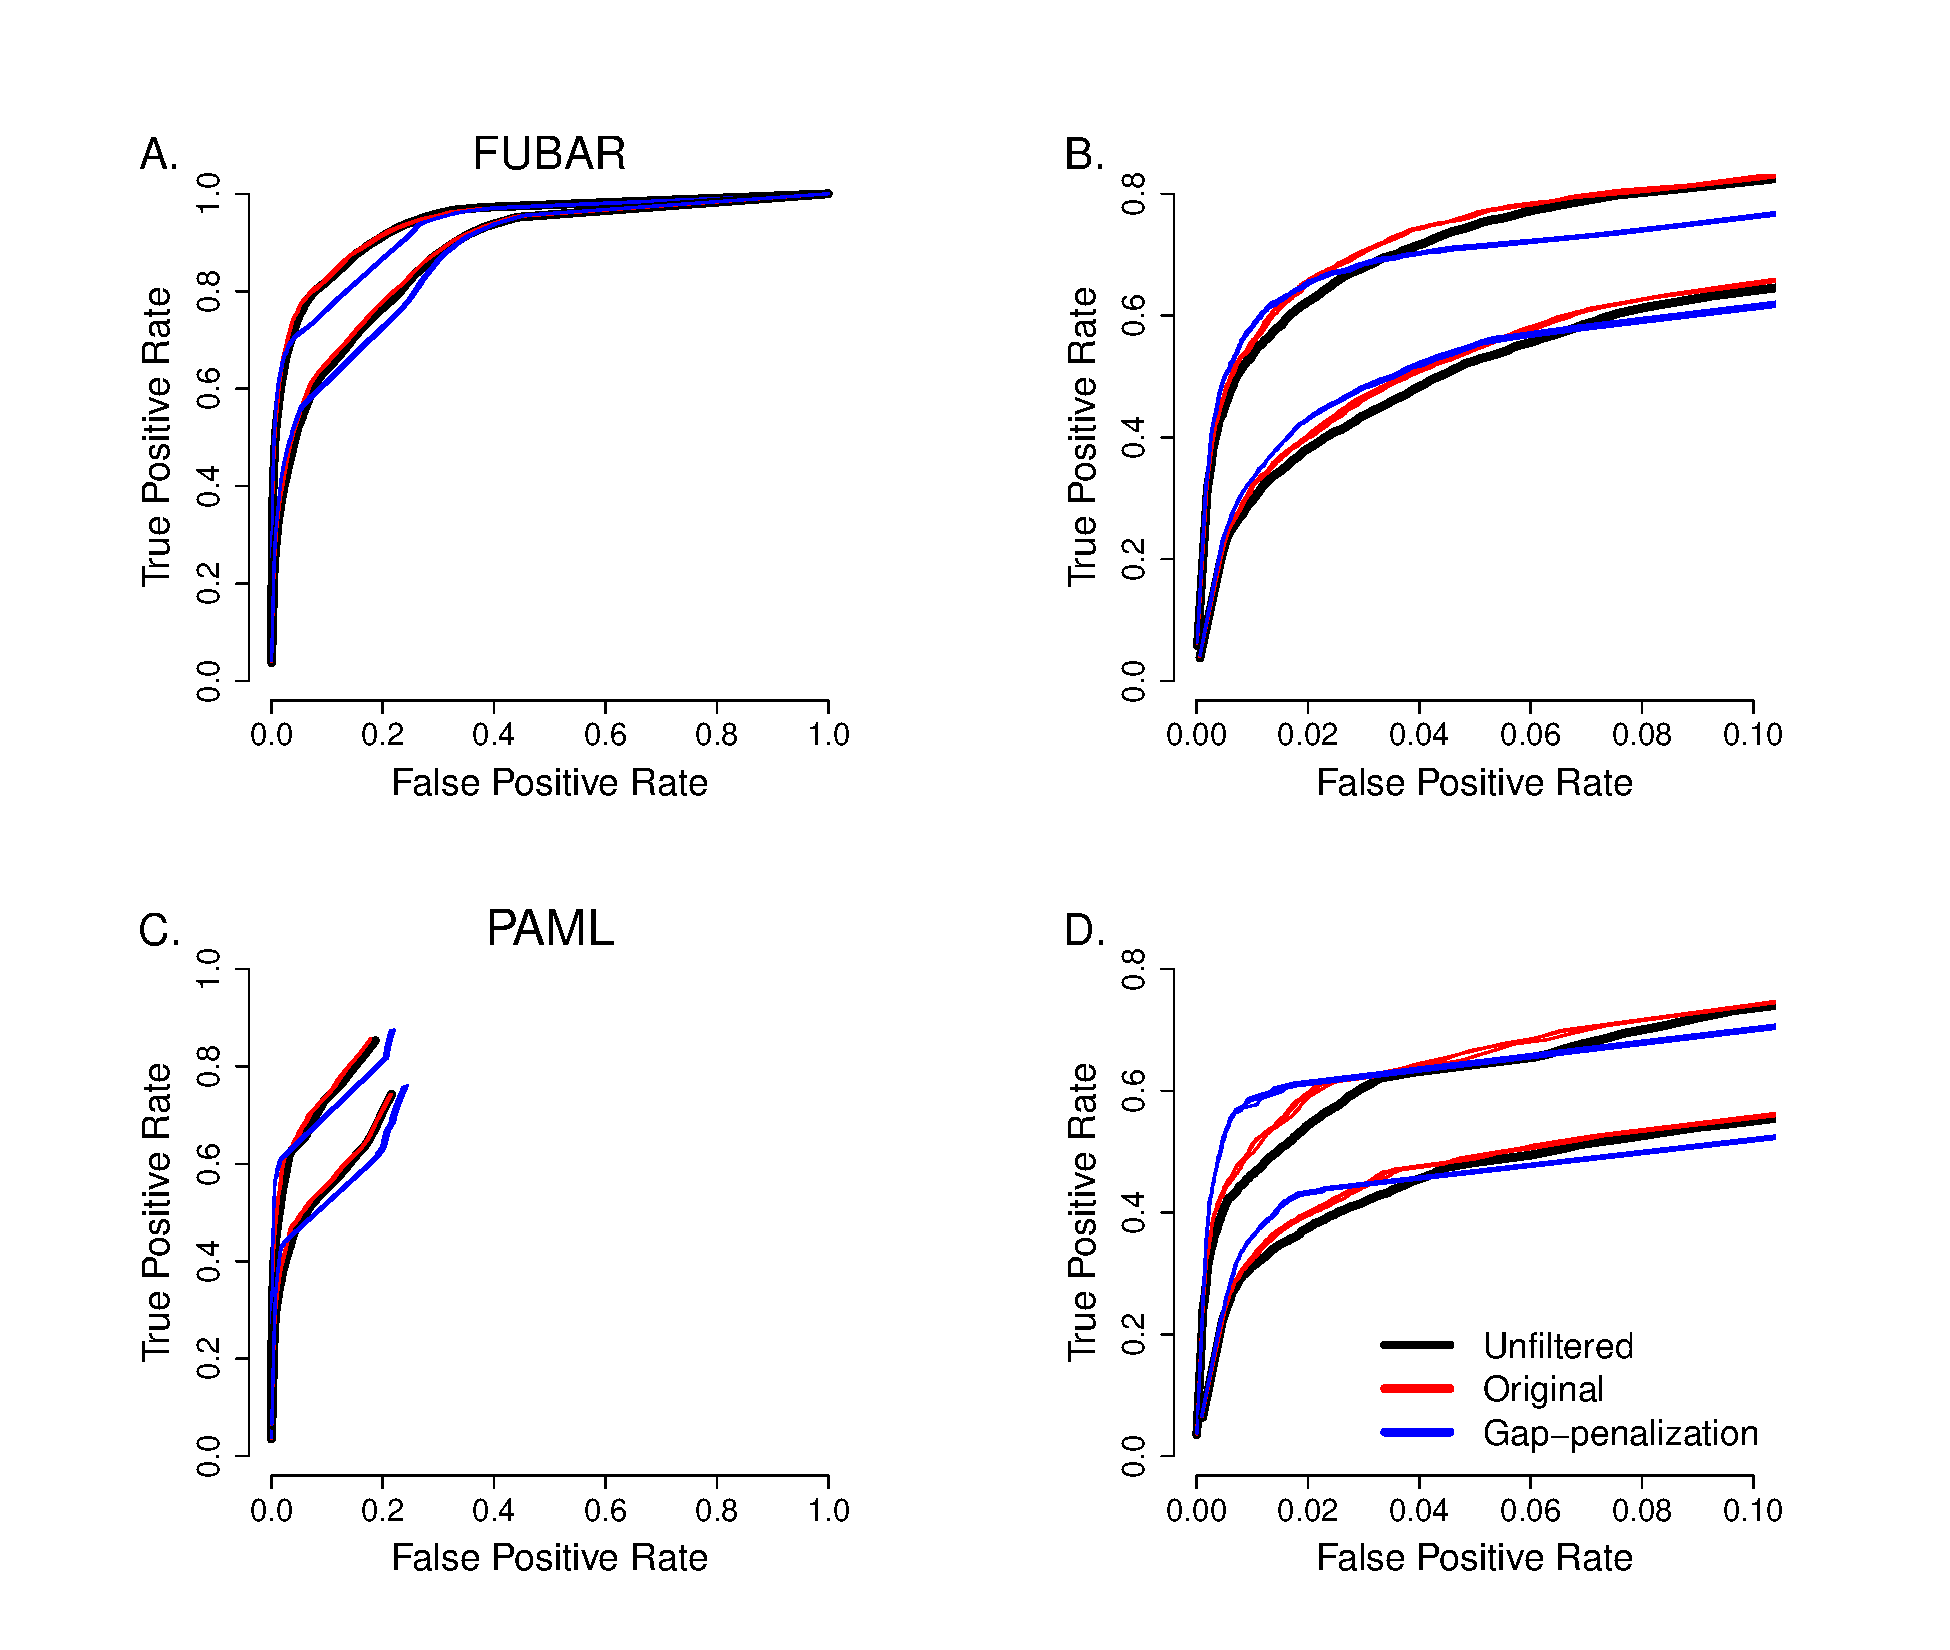
\includegraphics[width=6in]{Figures/ROC_prk.pdf}}
\caption{\label{roc} ROC curves as averaged across the two 60 sequence simulation sets. Within each panels, the top curve represents results from the HA selective profile, and the bottom curve represents results from the GP41 selective profile. Full ROC curves are shown in the left-hand panels. Note that, for the full PAML ROC curves, average FPRs higher than shown were not seen. The right-hand panels highlight specifically the low FPR regions (0--0.1) of the ROC curves. All MSA filtering algorithms (Guidance, BMweights, PDweights, GuidanceP, BMweightsP, and PDweightsP) are shown in ROC curves. A-B) ROC curves for positive-selection inference by FUBAR. C-D) ROC curves for positive-selection inference by PAML M8.}
\end{figure*}

\end{document}